\documentclass[aspectratio=169,10pt]{beamer}

\usetheme{metropolis}
\usecolortheme{default}

\usepackage[T1]{fontenc}
\usepackage[utf8]{inputenc}
\usepackage{newtxtext, newtxmath}   % Times-family text + math
\usepackage{microtype}
\usepackage{booktabs}
\usepackage{amsmath,amssymb}
\usepackage{graphicx}
\usepackage{xcolor}

\definecolor{luhblue}{RGB}{21,101,192}
\definecolor{alertred}{RGB}{198,40,40}
\definecolor{okgreen}{RGB}{27,94,32}
\definecolor{teal0}{RGB}{15,139,141}

\setbeamercolor{frametitle}{bg=luhblue, fg=white}
\setbeamercolor{progress bar}{fg=luhblue}
\setbeamercolor{alerted text}{fg=alertred}
\setbeamercolor{example text}{fg=okgreen}
\metroset{progressbar=frametitle, block=fill}

\graphicspath{{../paper_figs/}{../results/design_feedback/}}

\newcommand{\real}{\textcolor{okgreen}{\textbf{real data}}}
\newcommand{\synth}{\textcolor{alertred}{\textbf{synthetic}}}

\title{A Structure-Agnostic SHM Decision Framework\\for Reusable CFRP Spacecraft Structures}
\subtitle{from Real-Data Detection to Physics-Grounded Life Prognosis}
\author{K.\ Nishioka \and co-authors}
\institute{Keio University \quad / \quad Composites Part B (draft)}
\date{\today}

\begin{document}

\maketitle

% ------------------------------------------------------------------
\begin{frame}{The reusable-vehicle decision}
  \begin{columns}[T]
    \begin{column}{0.56\textwidth}
      Reusable launch vehicles change the SHM question:
      \begin{itemize}
        \item not ``did it survive one flight?''
        \item but \alert{may it fly again --- and for how many flights?}
      \end{itemize}
      \vspace{2mm}
      CFRP primary structures (interstage, fairing, motor case, tank, drive
      shaft) fail by \emph{internal} delamination / debond --- invisible,
      inferred from NDT.
      \vspace{2mm}

      \textbf{Gap:} no end-to-end pipeline that propagates uncertainty from
      detection to a re-flight decision \emph{and} states what real data supports.
    \end{column}
    \begin{column}{0.44\textwidth}
      \centering
      \footnotesize
      detect $\to$ classify $\to$ characterise\\
      $\to$ prognose $\to$ clear\\
      $\to$ fleet-learn $\to$ design
    \end{column}
  \end{columns}
\end{frame}

% ------------------------------------------------------------------
\begin{frame}{One decision core, five structures, four load modes}
  \centering
  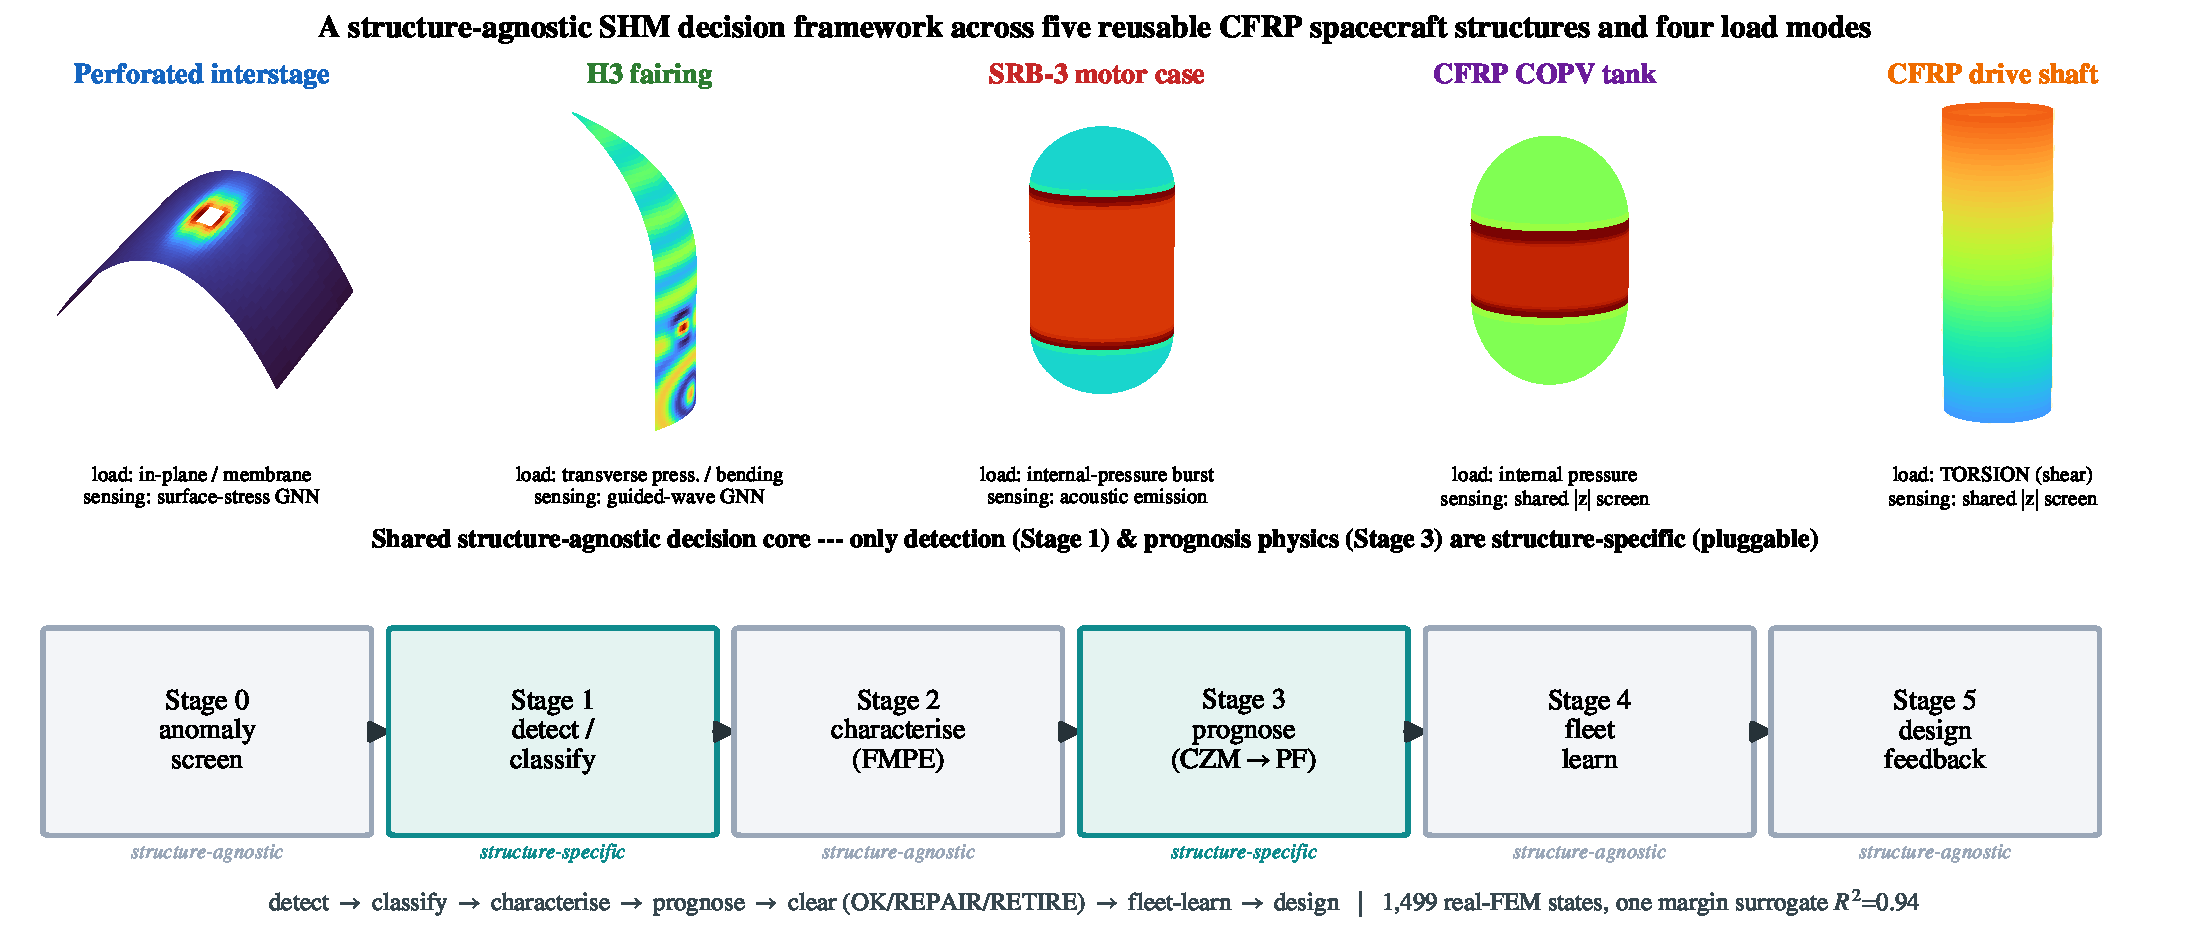
\includegraphics[width=0.96\textwidth]{framework_overview5.pdf}
  \vspace{1mm}
  \begin{itemize}\footnotesize
    \item Shared, structure-agnostic decision core (Stage 0/2/4/5 + clearance).
    \item Only \emph{detection} (Stage 1) and \emph{prognosis physics} (Stage 3)
          are structure-specific --- pluggable.
  \end{itemize}
\end{frame}

% ------------------------------------------------------------------
\begin{frame}{The five structures span the load-mode space}
  \centering\small
  \begin{tabular}{@{}lllc@{}}
    \toprule
    structure & load mode & detection front-end & evidence \\ \midrule
    interstage      & membrane          & surface-stress GNN & FEM + meas.\ TSA \\
    fairing         & transv./bending   & guided-wave GNN    & FEM + real OGW \\
    SRB-3 case      & pressure burst    & acoustic emission  & FEM + real AE \\
    \textbf{drive shaft} & \textbf{torsion} & shared $|z|$ (future) & CZM-FEM \\
    COPV tank       & int.\ pressure    & shared $|z|$ (future) & FEM \\
    \bottomrule
  \end{tabular}
  \vspace{3mm}
  \begin{itemize}\footnotesize
    \item Three demonstrated end-to-end with \real; two extend the load-mode
          coverage with FEM prognosis.
  \end{itemize}
\end{frame}

% ------------------------------------------------------------------
\begin{frame}{Detection front-ends --- grounded in real data}
  \begin{columns}[T]
    \begin{column}{0.5\textwidth}
      \centering
      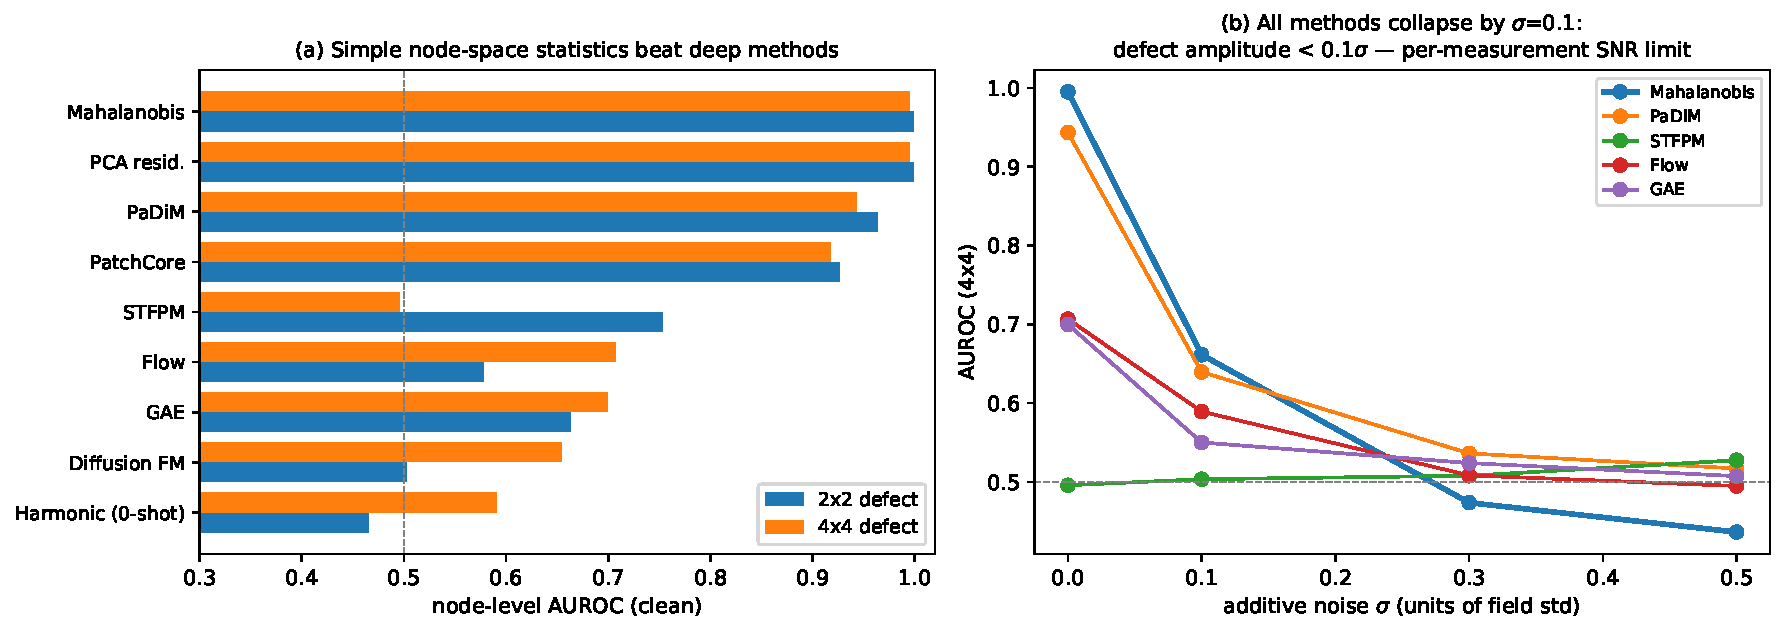
\includegraphics[width=\textwidth]{anomaly_zoo_benchmark.pdf}
      \footnotesize Stage-0 $|z|$ screen: per-node statistic dominates
      (AUROC $\approx0.99$, fixed geometry).
    \end{column}
    \begin{column}{0.5\textwidth}
      \footnotesize
      Structure-specific Stage-1 detectors:
      \begin{itemize}
        \item interstage: surface-stress GNN, macro-F1 $0.76$ (vs GAT $0.61$);
              detection generalises, localisation collapses OOD.
        \item fairing: guided-wave GNN, F1 $0.86$.
        \item SRB-3: real AE, per-hit AUROC $0.89$ / per-specimen $1.00$.
      \end{itemize}
    \end{column}
  \end{columns}
\end{frame}

% ------------------------------------------------------------------
\begin{frame}{How far does real data carry the pipeline? (honest)}
  \centering
  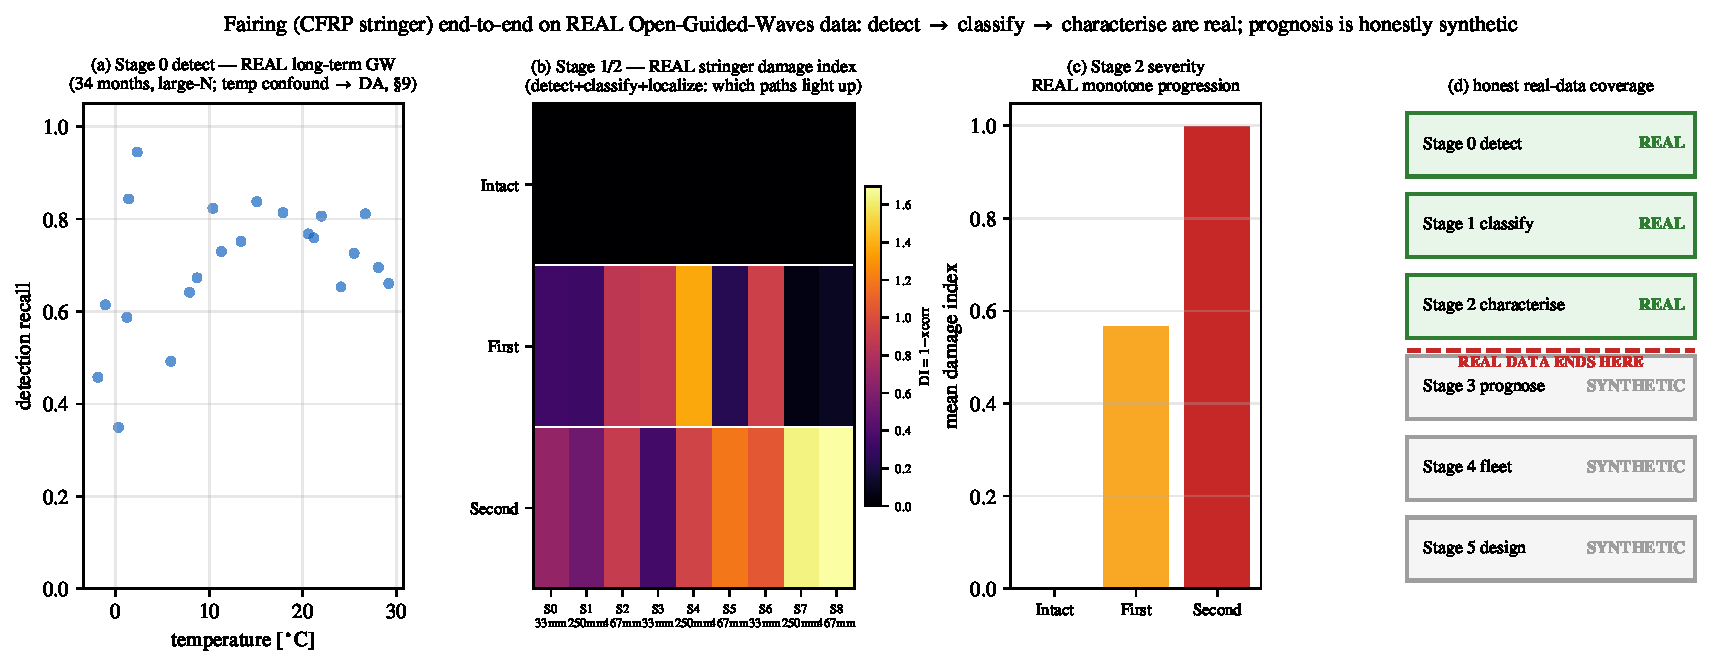
\includegraphics[width=0.95\textwidth]{fairing_real_e2e.pdf}
  \begin{itemize}\footnotesize
    \item Detect / classify / characterise on the fairing are \real{}
          (long-term guided waves, impact wavefield).
    \item \synth{} from Stage-3 prognosis onward (representative phase-field,
          synthetic fleet) --- the life side is the largest open gap.
  \end{itemize}
\end{frame}

% ------------------------------------------------------------------
\begin{frame}{Structure-agnostic core --- and its boundary}
  \begin{columns}[T]
    \begin{column}{0.6\textwidth}
      \centering
      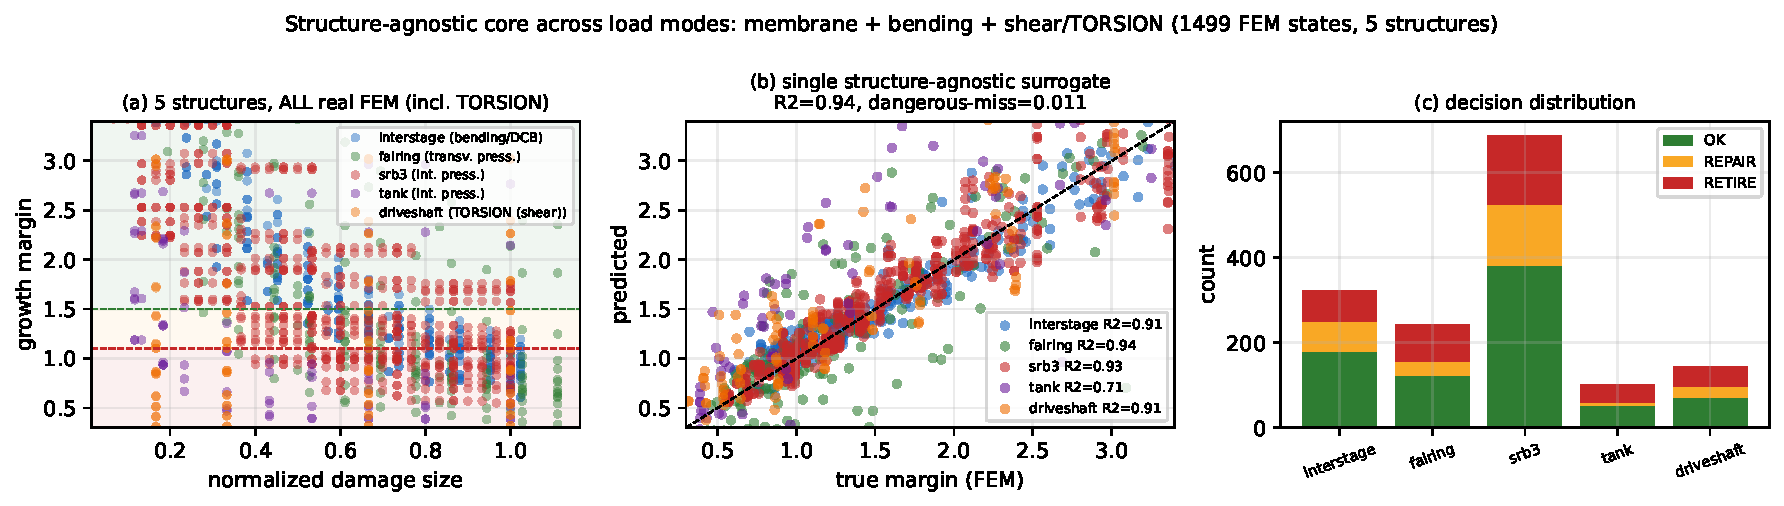
\includegraphics[width=\textwidth]{structure_agnostic_loso.pdf}
    \end{column}
    \begin{column}{0.4\textwidth}
      \footnotesize
      A single margin surrogate over \textbf{1{,}499 real-FEM} critical-load
      states fits all five ($R^2{=}0.94$, dangerous-miss $1.1\%$).
      \vspace{2mm}

      \alert{Honest boundary:} leave-one-\emph{load-mode}-out to the unseen
      torsion shaft \emph{fails} ($R^2<0$).
      \vspace{1mm}

      \textbf{Geometry transfers; load mode does not.}
    \end{column}
  \end{columns}
\end{frame}

% ------------------------------------------------------------------
\begin{frame}{New load mode: the CFRP torsion drive shaft}
  \begin{columns}[T]
    \begin{column}{0.5\textwidth}
      \centering
      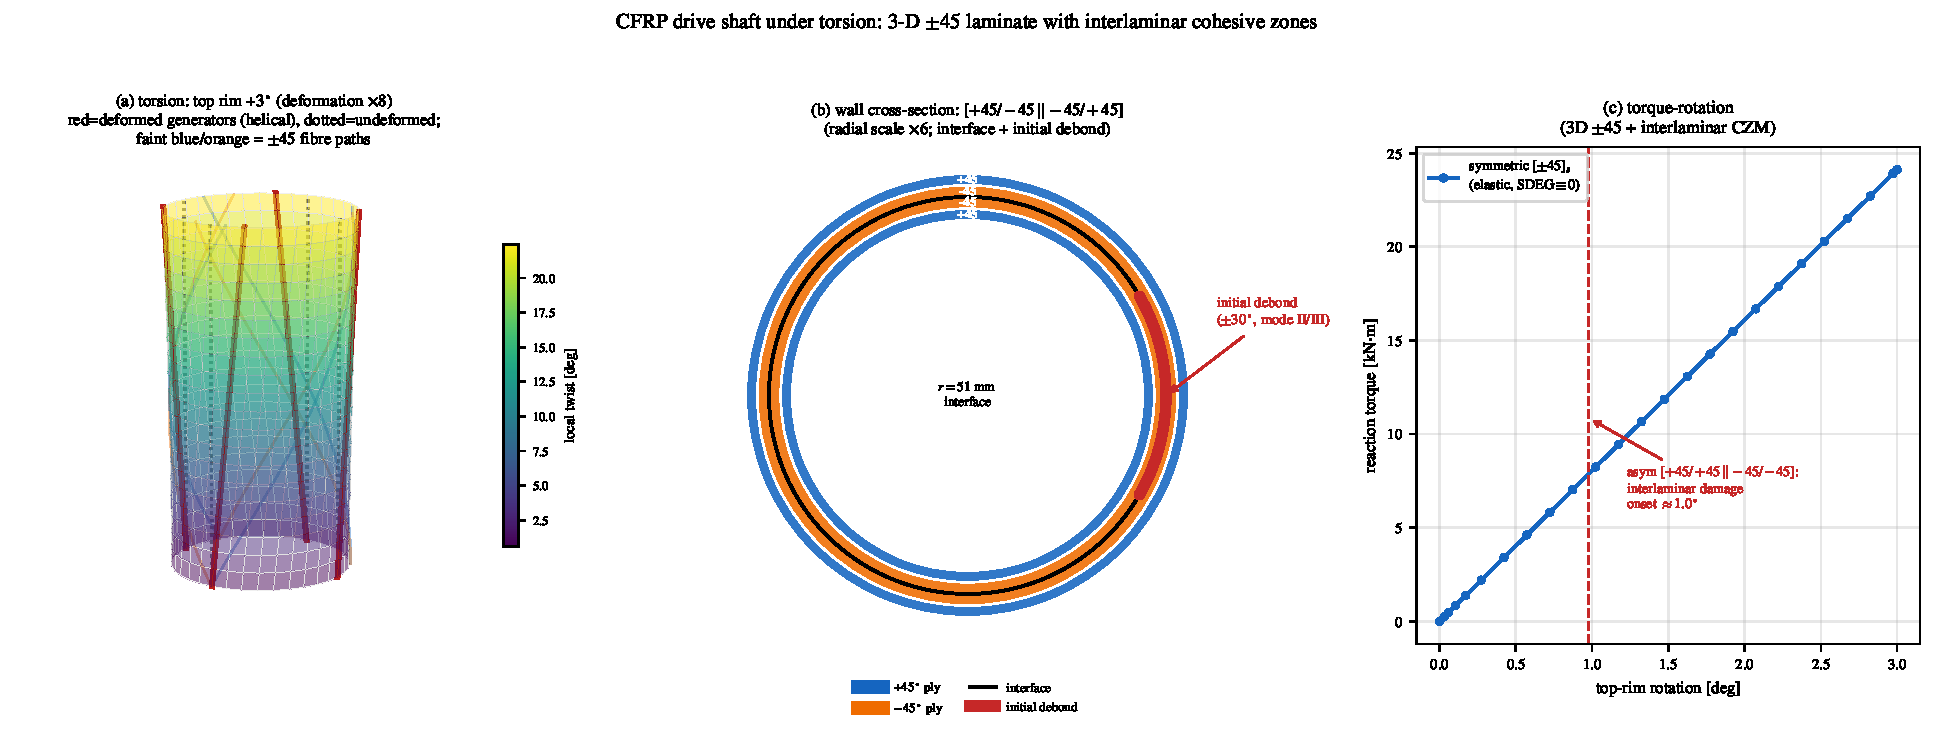
\includegraphics[width=\textwidth]{shaft_torsion_3d.pdf}\\
      \footnotesize CGAX screen: $\pm45$ tube, groove damage, $T_{cr}$ sweep.
    \end{column}
    \begin{column}{0.5\textwidth}
      \centering
      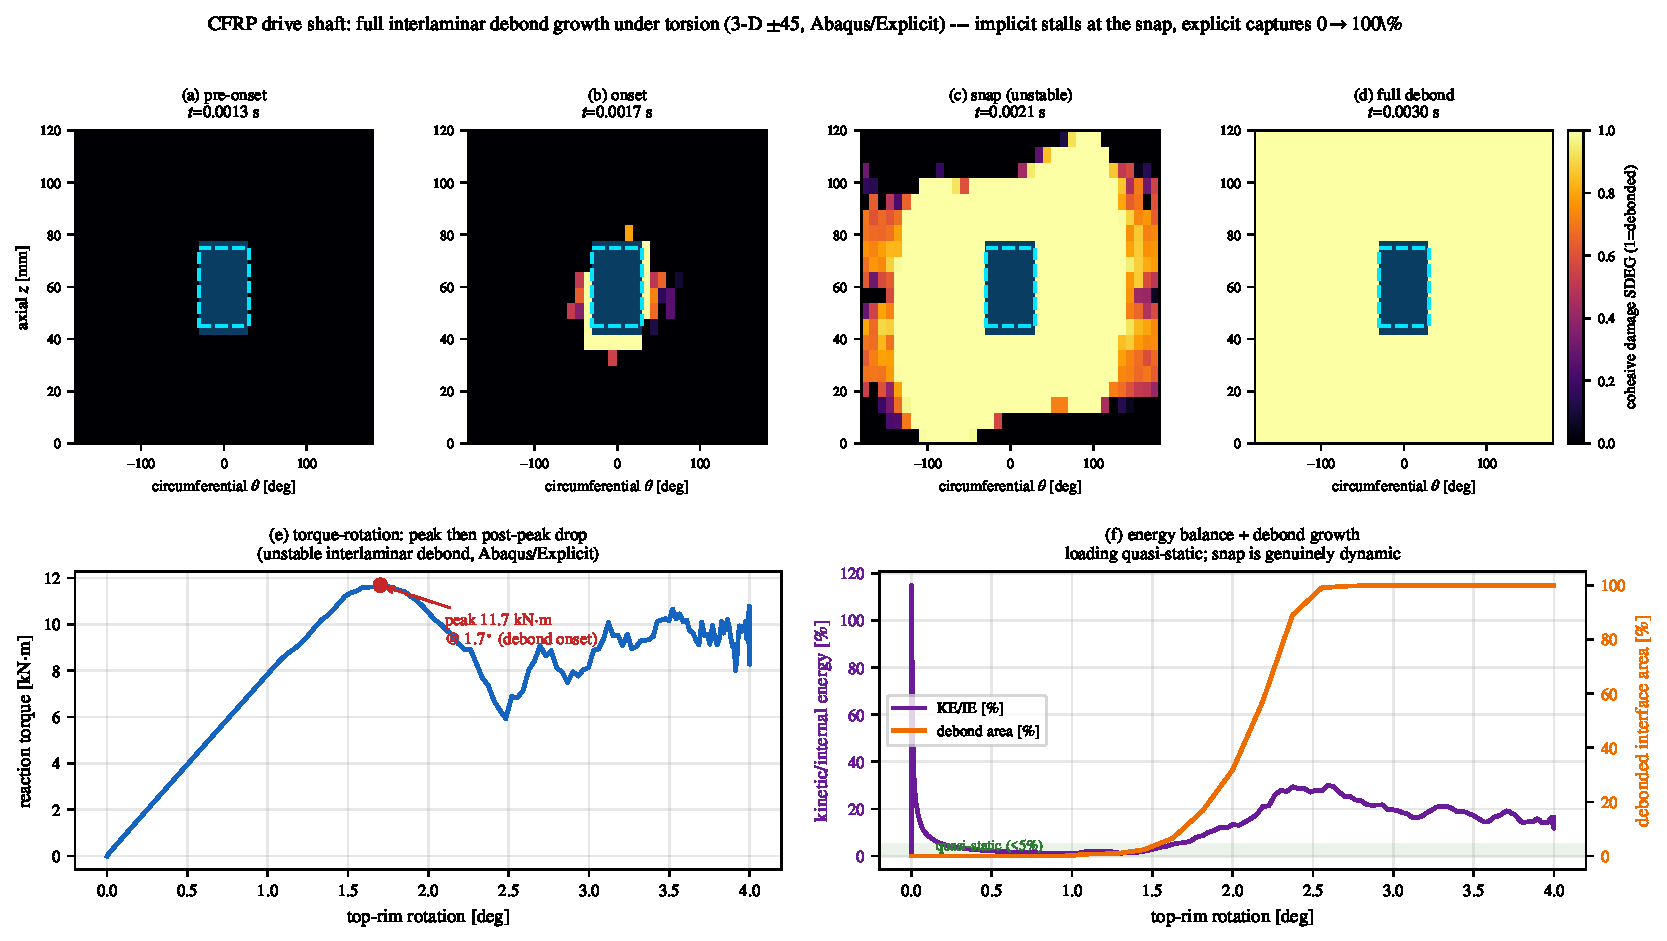
\includegraphics[width=\textwidth]{shaft_explicit_debond.pdf}\\
      \footnotesize 3-D $\pm45$ + interlaminar CZM: full $0\to100\%$ debond.
      Implicit stalls at the snap; \textbf{explicit} captures it.
    \end{column}
  \end{columns}
\end{frame}

% ------------------------------------------------------------------
\begin{frame}{End-to-end decision reliability (vs a \synth{} oracle)}
  \begin{columns}[T]
    \begin{column}{0.58\textwidth}
      \centering
      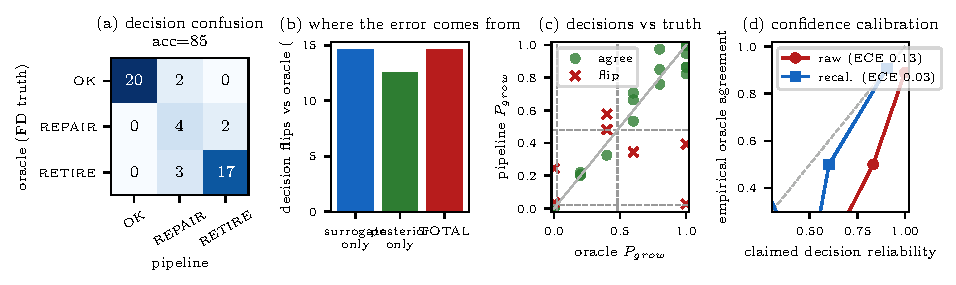
\includegraphics[width=\textwidth]{decision_uq.pdf}
    \end{column}
    \begin{column}{0.42\textwidth}
      \footnotesize
      Propagate uncertainty to the clearance call; score against the exact
      FD-physics oracle.
      \begin{itemize}
        \item accuracy \textbf{85\%}, dangerous-miss \textbf{0\%}
        \item Platt recalibration: ECE $0.18\!\to\!0.06$
      \end{itemize}
      \alert{Measured against a synthetic oracle} --- internal error
      propagation, not agreement with real life tests.
    \end{column}
  \end{columns}
\end{frame}

% ------------------------------------------------------------------
\begin{frame}{Sim-to-real: normalisation choice controls false alarms}
  \begin{columns}[T]
    \begin{column}{0.55\textwidth}
      \centering
      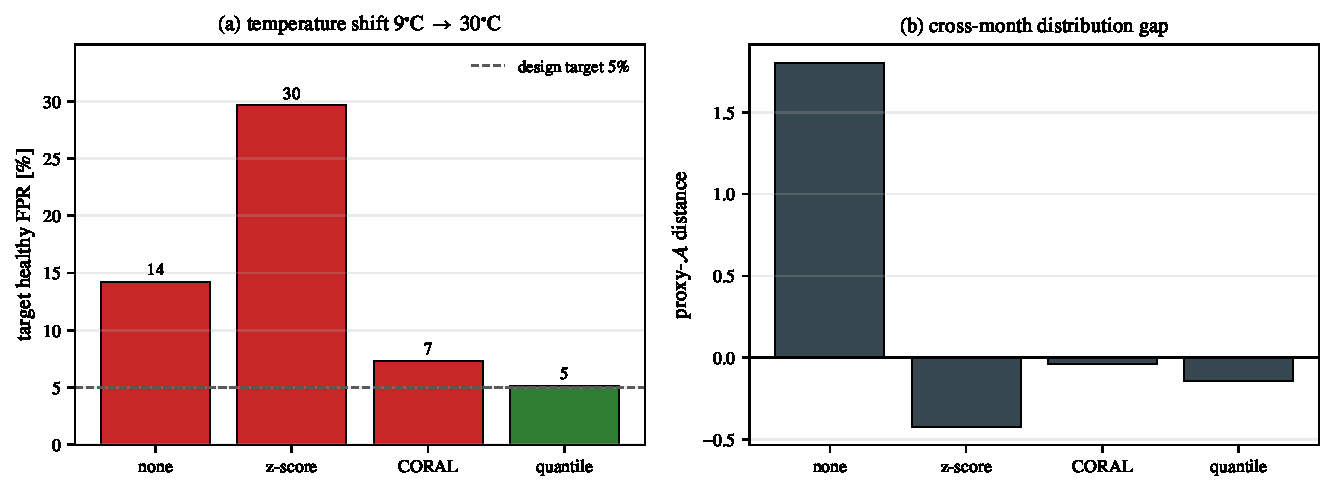
\includegraphics[width=\textwidth]{payload_da_longterm.pdf}
    \end{column}
    \begin{column}{0.45\textwidth}
      \footnotesize
      Real OGW temperature shift $9^\circ\!\to\!30^\circ$C:
      \begin{itemize}
        \item uncorrected FPR \textbf{14\%} (temperature mimics damage)
        \item quantile DA $\to$ \textcolor{okgreen}{\textbf{5\%}} (design target)
        \item \alert{z-score normalisation worsens to 30\%}
      \end{itemize}
      Interstage TSA: quantile DA closes 97\% of the gap.
    \end{column}
  \end{columns}
\end{frame}

% ------------------------------------------------------------------
\begin{frame}{Stage-5 design feedback --- mechanism, not a calibrated value}
  \begin{columns}[T]
    \begin{column}{0.6\textwidth}
      \centering
      
\includegraphics[width=\textwidth]{design_robustness.pdf}
    \end{column}
    \begin{column}{0.4\textwidth}
      \footnotesize
      Fleet-driven inverse design steers off-axis angle + interface toughness.
      \vspace{2mm}

      \alert{Honest limitation:} under uncalibrated phase-field constants the
      optimal angle spans $15^\circ$--$75^\circ$ --- leverage exists only near
      the growth transition.
      \vspace{1mm}

      The \textbf{mechanism} is robust; a quoted optimum needs calibration.
    \end{column}
  \end{columns}
\end{frame}

% ------------------------------------------------------------------
\begin{frame}{Honest accounting}
  \begin{itemize}
    \item \real{}: detection / classification / characterisation
          (guided waves, AE, TSA), posterior coverage, $1{,}499$-state FEM core.
    \item \synth{}: prognosis, clearance, fleet, design --- representative
          phase-field + synthetic fleets; decision UQ vs a synthetic oracle.
    \item \alert{Largest gap:} no real life-test validation of the life side.
    \item Priority inputs: Kojima TSA full-field (interstage), real fatigue data.
  \end{itemize}
\end{frame}

% ------------------------------------------------------------------
\begin{frame}{Bridge to the Keio continuation}
  \begin{itemize}
    \item The differentiable, fast forward (FNO; autograd-exact) is what a
          TMCMC / Bayesian-inverse phase needs.
    \item Its physics --- anisotropic phase-field seeded by interlaminar
          cohesive zones --- is the prognosis layer the torsion shaft extends
          from mode-I to mode-II/III shear.
    \item[$\Rightarrow$] \textbf{Phase-field $\times$ GNN prognosis}, calibrated
          on measured data, is the computational-solid-mechanics continuation.
  \end{itemize}
\end{frame}

% ------------------------------------------------------------------
\begin{frame}[standout]
  One decision core across four load modes.\\[2mm]
  Real where data permits, honest where it does not.\\[2mm]
  Closing the life-side real-data gap is next.
\end{frame}

% ==================================================================
\appendix

\begin{frame}[standout]
  Appendix / backup
\end{frame}

% --- A1 ---
\begin{frame}{A1 --- Stage-0 anomaly benchmark (clean, fixed geometry)}
  \centering\small
  \begin{tabular}{@{}lcc@{}}
    \toprule method & 2$\times$2 & 4$\times$4 \\ \midrule
    per-node Mahalanobis & 0.999 & 0.995 \\
    PCA residual         & 0.999 & 0.995 \\
    PaDiM                & 0.964 & 0.944 \\
    PatchCore            & 0.927 & 0.918 \\
    STFPM                & 0.754 & 0.496 \\
    graph autoencoder    & 0.663 & 0.700 \\
    flow (RealNVP)       & 0.578 & 0.707 \\
    diffusion (FM)       & 0.503 & 0.663 \\
    harmonicity (0-shot) & 0.465 & 0.590 \\ \bottomrule
  \end{tabular}\\[1mm]
  \footnotesize node-level AUROC. Per-node statistics dominate on fixed geometry;
  the defect sits below $0.1\sigma$ (a per-measurement SNR limit).
\end{frame}

% --- A2 ---
\begin{frame}{A2 --- Decision rule and launch economics}
  \begin{columns}[T]
    \begin{column}{0.5\textwidth}
      \centering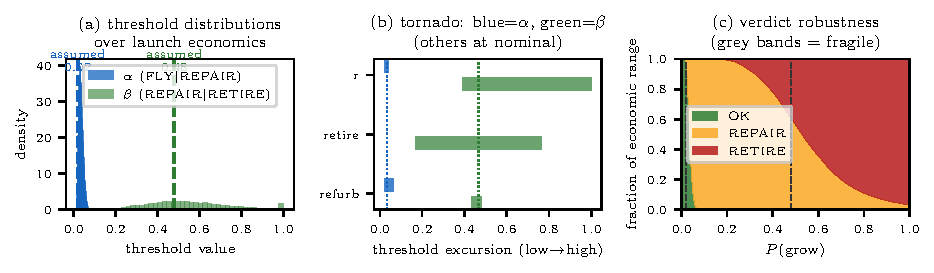
\includegraphics[width=\textwidth]{cost_calibration.pdf}
    \end{column}
    \begin{column}{0.5\textwidth}\footnotesize
      $a^\star=\arg\min_a \mathbb{E}_{p(\theta\mid x)}[C(a,\theta)]$, actions
      \{OK, REPAIR, RETIRE\}.
      \begin{itemize}
        \item MC over refurb/loss $1/100$--$1/30$, retire/loss $0.1$--$0.4$
        \item $\alpha=0.035\,[0.021,0.055]$, $\beta=0.53\,[0.28,0.93]$
        \item REPAIR-vs-RETIRE flips at $P_{\text{grow}}\!\approx\!0.3$--$0.5$
              (economics-fragile)
      \end{itemize}
    \end{column}
  \end{columns}
\end{frame}

% --- A3 ---
\begin{frame}{A3 --- Stage-2 characterisation (FMPE) vs differentiable physics}
  \centering\small
  \begin{tabular}{@{}llccc@{}}
    \toprule set & method & $c_x$ RMSE & size RMSE & 90\% cov.\ \\ \midrule
    in-dist & FMPE      & 0.006 & 0.002 & 0.958 \\
    in-dist & diff-phys & 0.001 & 0.003 & 1.000 \\
    OOD     & FMPE      & \textbf{0.144} & \textbf{0.096} & \textbf{0.000} \\
    OOD     & diff-phys & 0.002 & 0.001 & 0.958 \\ \bottomrule
  \end{tabular}\\[1mm]
  \footnotesize Forward physics generalises; amortised inference extrapolates
  poorly $\Rightarrow$ hybrid Stage-2 (amortised in-dist, physics-grounded OOD).
\end{frame}

% --- A4 ---
\begin{frame}{A4 --- Stage-3 prognosis: anisotropic phase-field}
  \footnotesize
  \[
  \Psi(\mathbf u,d)=\!\int_\Omega\!\Big[g(d)\psi^{+}(\boldsymbol\varepsilon)
  +\tfrac{G_c}{c_w}\Big(\tfrac{d^2}{\ell}+\ell\,\nabla d\!\cdot\!\mathbf A\nabla d\Big)\Big]d\Omega
  \]
  \begin{itemize}
    \item $\mathbf A=\mathbf I+\beta\,\mathbf a\!\otimes\!\mathbf a$: fibre-aligned crack resistance;
          interface $G_c^{\text{int}}/G_c^{\text{ply}}\!\approx\!0.3$--$0.6$ (DCB/ENF anchored).
    \item Carrara-2020 fatigue history degrades $G_c$ across flights (no i.i.d.\ shortcut).
    \item Pluggable: fairing skin-core debond ($G=\kappa\sigma^2a^2$, Paris);
          SRB-3 burst; \emph{torsion} interlaminar CZM.
  \end{itemize}
\end{frame}

% --- A4b ---
\begin{frame}{A4b --- Does a remaining-life clock exist? (real-data validated)}
  \centering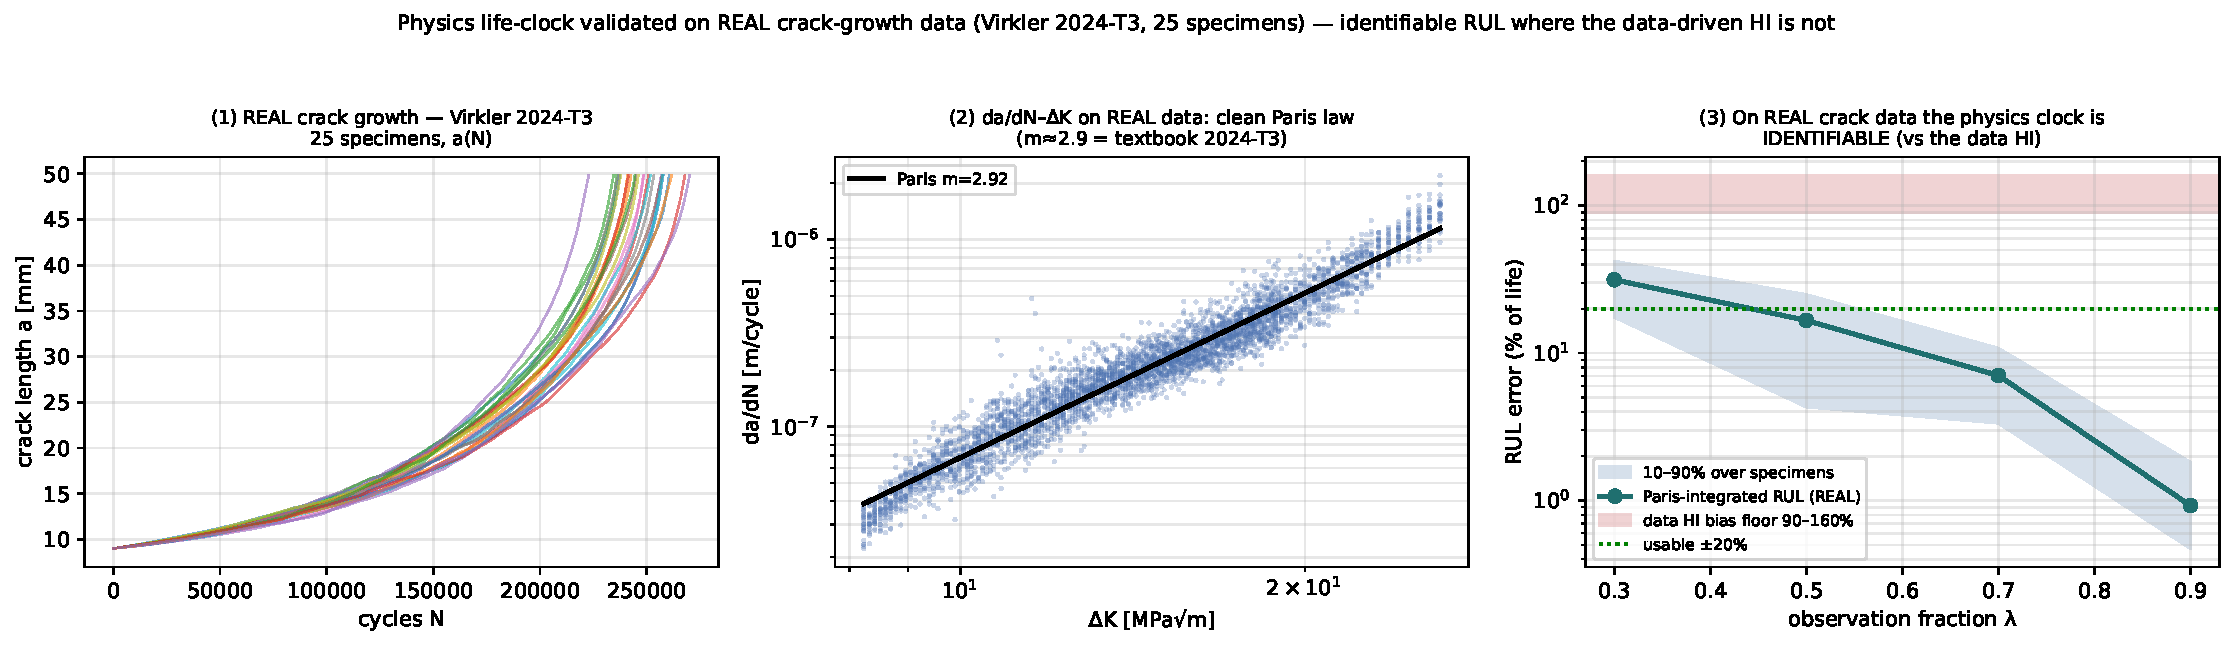
\includegraphics[width=0.95\textwidth]{virkler_validation.pdf}\\[2pt]
  \begin{itemize}\footnotesize
    \item \textbf{Data-driven} health index: \emph{no} usable clock --- point-RUL bias floor
          $90$--$160\%$ of life (real ReMAP DFOS); no reframing rescues it.
    \item \textbf{Physical} Paris/phase-field clock: identifiable, validated on \emph{real} crack
          growth --- Virkler 2024-T3 ($m{=}2.92$), RUL error $16.7\%\!\to\!0.9\%$ as $\lambda$ grows.
    \item Real CFRP DCB: identifiable per-specimen but coarser --- fibre bridging breaks the single
          $\mathrm{d}a/\mathrm{d}N$--$\Delta G$ law ($m\!\approx\!17$).
    \item Same estimator: fails on the data index, works on the physics clock $\Rightarrow$ the
          life-side limit is the \textbf{signal}, not the method.
  \end{itemize}
\end{frame}

% --- A5 ---
\begin{frame}{A5 --- Fast surrogate + trust gate}
  \begin{columns}[T]
    \begin{column}{0.5\textwidth}
      \centering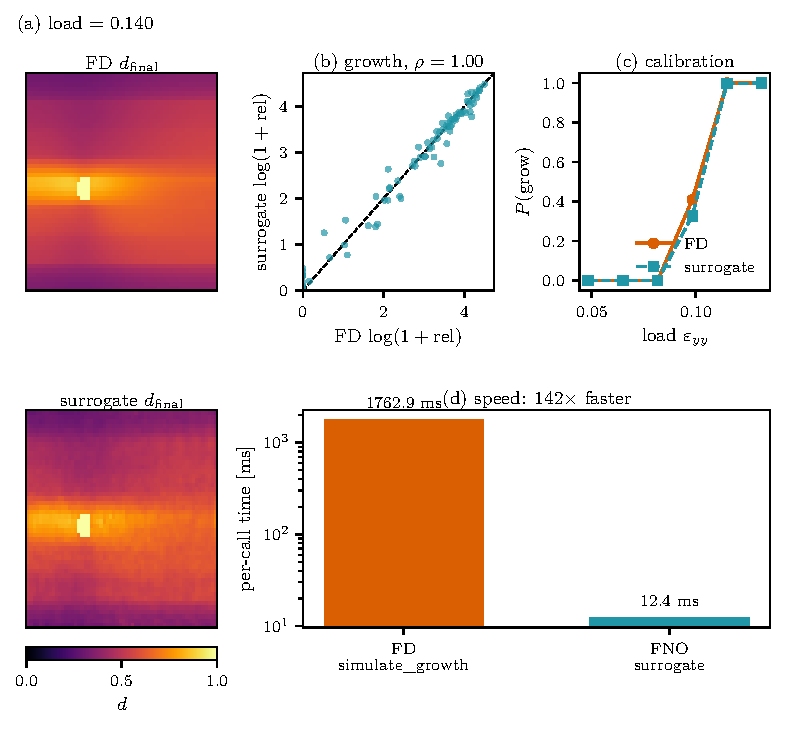
\includegraphics[width=\textwidth]{crack_surrogate.pdf}\\
      \footnotesize FNO: field rel-$L_2$ $3.5\%$, grow-flag $0.988$, \textbf{142$\times$} speed.
    \end{column}
    \begin{column}{0.5\textwidth}
      \centering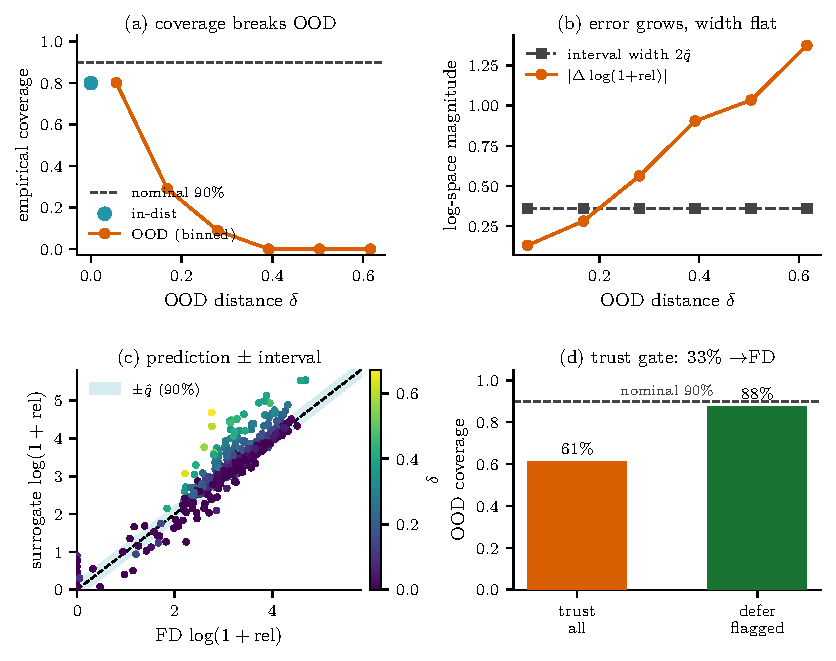
\includegraphics[width=\textwidth]{conformal_surrogate.pdf}\\
      \footnotesize Split-conformal trust gate: flags $33\%$ of an OOD stream,
      restores coverage $61\%\!\to\!88\%$.
    \end{column}
  \end{columns}
\end{frame}

% --- A6 ---
\begin{frame}{A6 --- Structure-agnostic surrogate: details}
  \begin{columns}[T]
    \begin{column}{0.55\textwidth}
      \centering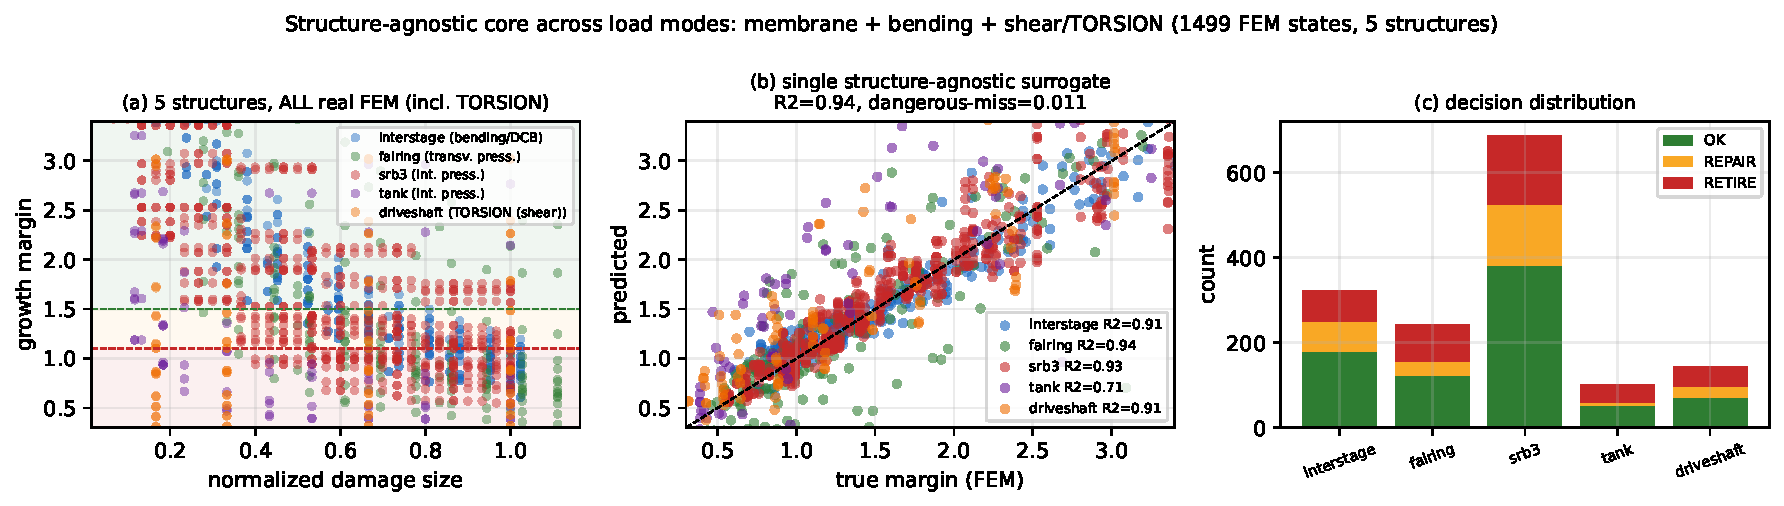
\includegraphics[width=\textwidth]{structure_agnostic_loso.pdf}
    \end{column}
    \begin{column}{0.45\textwidth}\footnotesize
      $1{,}499$ real-FEM states; descriptors [dmg, crit, aux, stiffness] + structure one-hot.
      \begin{itemize}
        \item per-structure $R^2$: interstage 0.91, fairing 0.94, SRB-3 0.93,
              tank 0.71, drive shaft 0.91
        \item shared rule: acc 0.86, dangerous-miss $1.1\%$
        \item LOSO torsion: $R^2=-1.4$, dangerous-miss $17\%$ (load-mode boundary)
      \end{itemize}
    \end{column}
  \end{columns}
\end{frame}

% --- A7 ---
\begin{frame}{A7 --- Torsion shaft: CGAX screen + 3-D explicit CZM}
  \begin{columns}[T]
    \begin{column}{0.5\textwidth}\footnotesize
      \textbf{CGAX screen} ($\pm45$ tube, twist DOF):
      \begin{itemize}
        \item analytic check: wall shear $17.1$ vs $T/2\pi R^2t=16.8$ MPa
        \item $144$-state groove sweep, $T_{cr}$ $0.31$--$7.76$ kN$\cdot$m
        \item true torsional buckling is non-axisymmetric $\Rightarrow$ 3-D
      \end{itemize}
    \end{column}
    \begin{column}{0.5\textwidth}
      \centering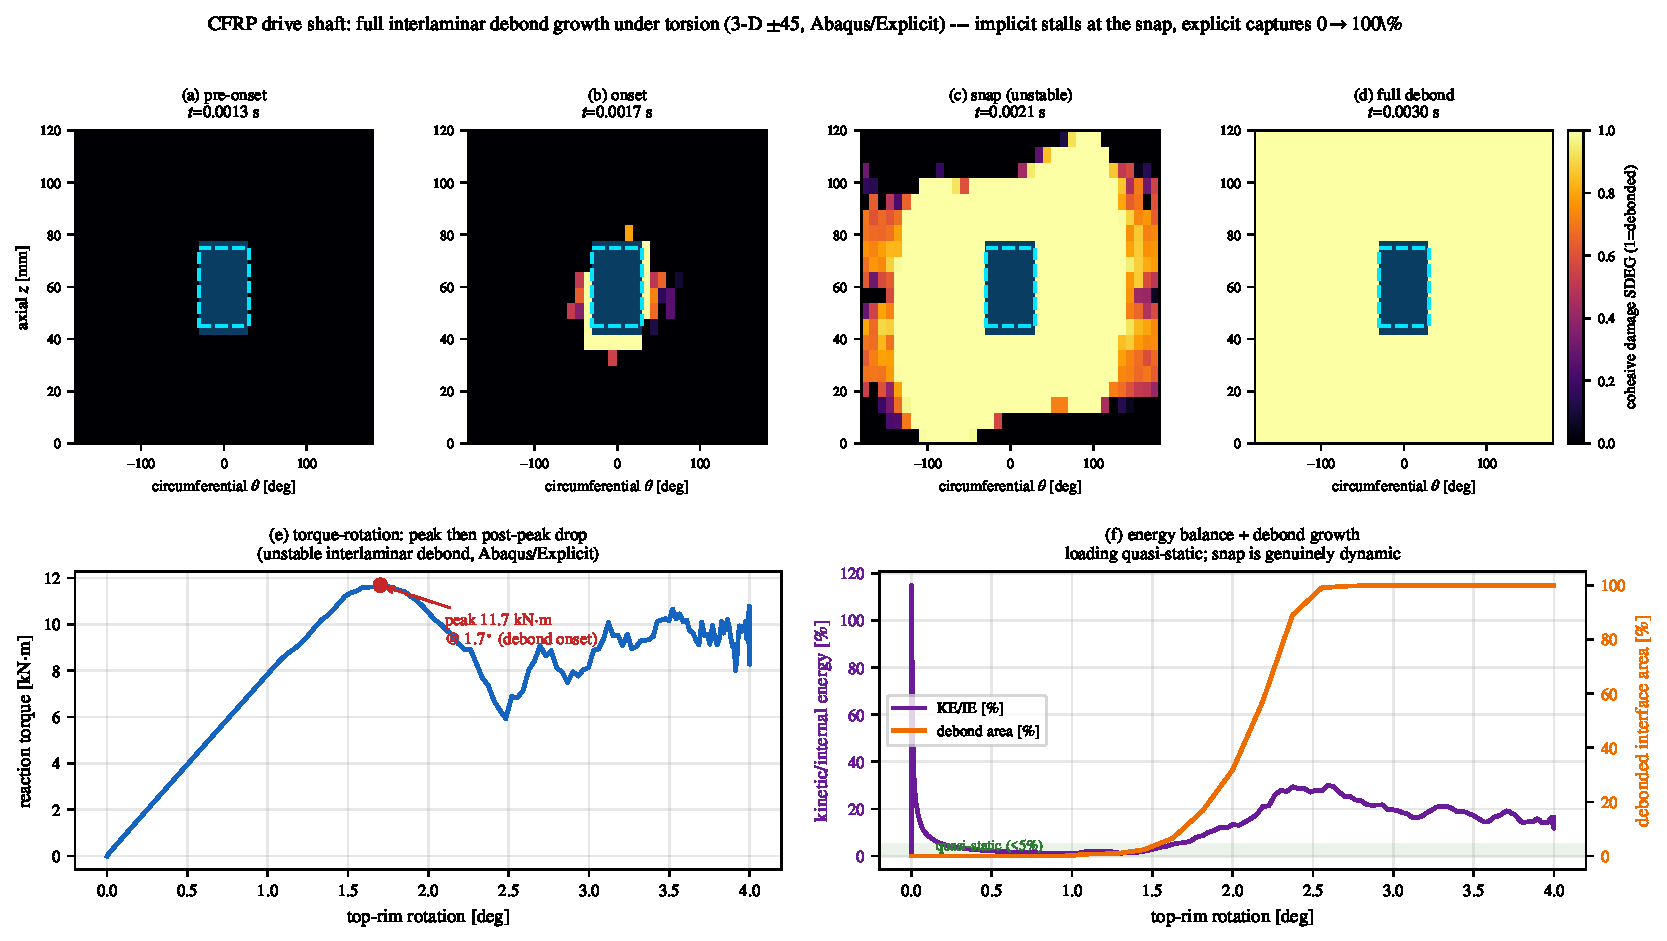
\includegraphics[width=\textwidth]{shaft_explicit_debond.pdf}\\
      \footnotesize 3-D explicit: KE/IE $1.3$--$3.6\%$ in loading (quasi-static),
      peak $11.7$ kN$\cdot$m @ $1.7^\circ$, debond $0\!\to\!100\%$.
    \end{column}
  \end{columns}
\end{frame}

% --- A8 ---
\begin{frame}{A8 --- SRB-3 acoustic-emission detection (real data)}
  \begin{columns}[T]
    \begin{column}{0.52\textwidth}
      \centering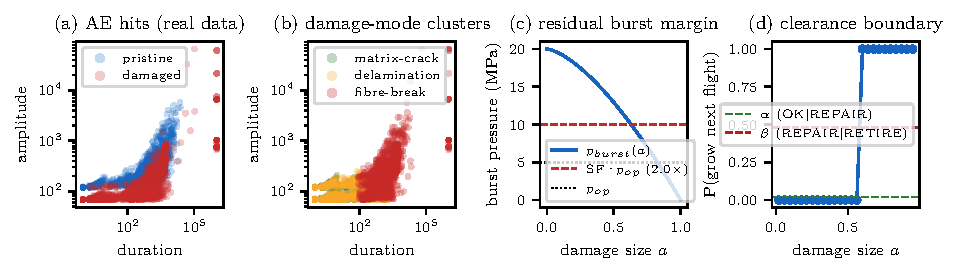
\includegraphics[width=\textwidth]{srb3_motorcase.pdf}
    \end{column}
    \begin{column}{0.48\textwidth}\footnotesize
      4TU CC0 AE, $\sim$$48$k Vallen hits:
      \begin{itemize}
        \item group-aware RF: per-hit AUROC $0.888$ / per-specimen $1.000$
              (linear baseline $\sim$$0.52$)
        \item amplitude--duration damage-mode clustering
      \end{itemize}
      \alert{Honest:} compression-pristine coupons also emit high-energy AE
      $\Rightarrow$ the multivariate detector, not one cluster, is the read-out;
      AE is a real-data \emph{proxy} for the motor-case front-end.
    \end{column}
  \end{columns}
\end{frame}

% --- A9 ---
\begin{frame}{A9 --- Sim-to-real domain adaptation: details}
  \begin{columns}[T]
    \begin{column}{0.5\textwidth}
      \centering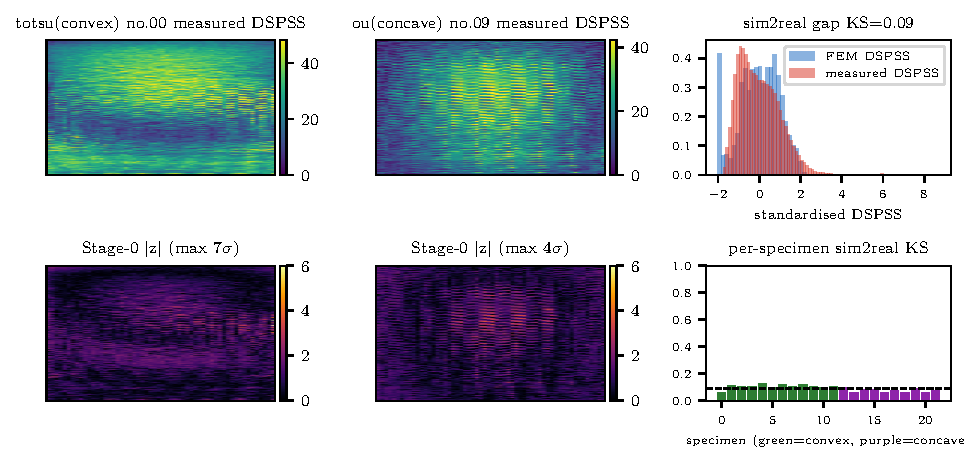
\includegraphics[width=\textwidth]{tsa_sim2real.pdf}\\
      \footnotesize Interstage TSA: proxy-$\mathcal A$ $2.0\!\to\!0.3$ ($97\%$ closed).
    \end{column}
    \begin{column}{0.5\textwidth}
      \centering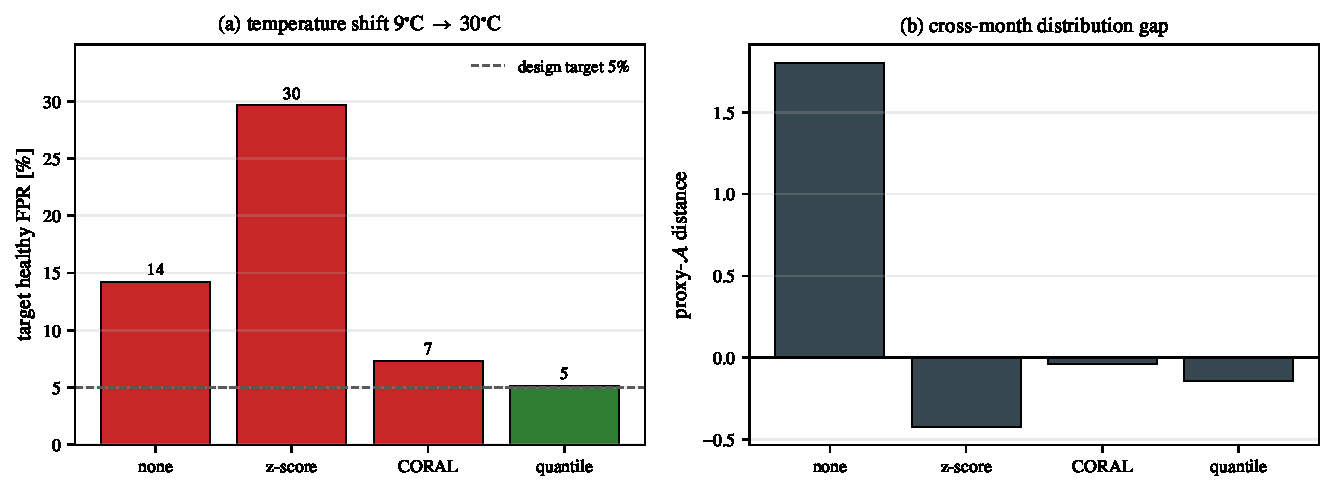
\includegraphics[width=\textwidth]{payload_da_longterm.pdf}\\
      \footnotesize Fairing OGW: FPR $14\!\to\!5\%$ (quantile), CORAL $7\%$,
      z-score $\to$ $30\%$; threshold set on source healthy (no target leak).
    \end{column}
  \end{columns}
\end{frame}

% --- A10 ---
\begin{frame}{A10 --- End-to-end decision UQ: error decomposition}
  \begin{columns}[T]
    \begin{column}{0.55\textwidth}
      \centering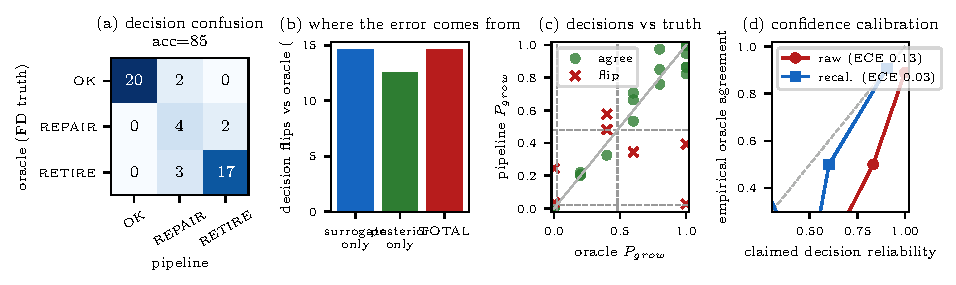
\includegraphics[width=\textwidth]{decision_uq.pdf}
    \end{column}
    \begin{column}{0.45\textwidth}\footnotesize
      Four decisions isolate each error (over 40 held-out scenarios):
      \begin{itemize}
        \item Stage-2 posterior: flip rate $25\%$ (dominant)
        \item surrogate forward: $17.5\%$
        \item partial cancellation $\to$ total $15\%$
        \item all $16$ RETIRE cases caught (0\% dangerous-miss)
      \end{itemize}
      Oracle = exact FD physics (\synth).
    \end{column}
  \end{columns}
\end{frame}

% --- A11 ---
\begin{frame}{A11 --- Solver verification and robustness}
  \begin{columns}[T]
    \begin{column}{0.55\textwidth}
      \centering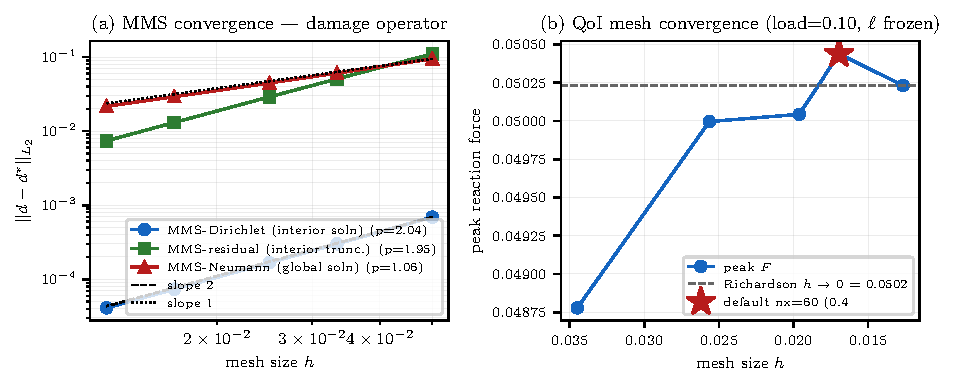
\includegraphics[width=\textwidth]{physics_validation.pdf}
    \end{column}
    \begin{column}{0.45\textwidth}\footnotesize
      \begin{itemize}
        \item MMS: interior order $2.04$ (2-D), $2.05$ (3-D)
        \item mesh convergence: $0.4\%$ at $n_x{=}60$
        \item constant-peak proxy under-predicts life $3.4\times$ vs a variable
              flight spectrum (S--N anchored)
        \item Stage-0 holds AUROC $0.84$ at $\sigma{=}0.1$; chance near
              $\sigma\!\approx\!0.7$--$1.0$
      \end{itemize}
    \end{column}
  \end{columns}
\end{frame}

% --- A12 ---
\begin{frame}{A12 --- Stage-4 hierarchical fleet learning}
  \begin{columns}[T]
    \begin{column}{0.55\textwidth}
      \centering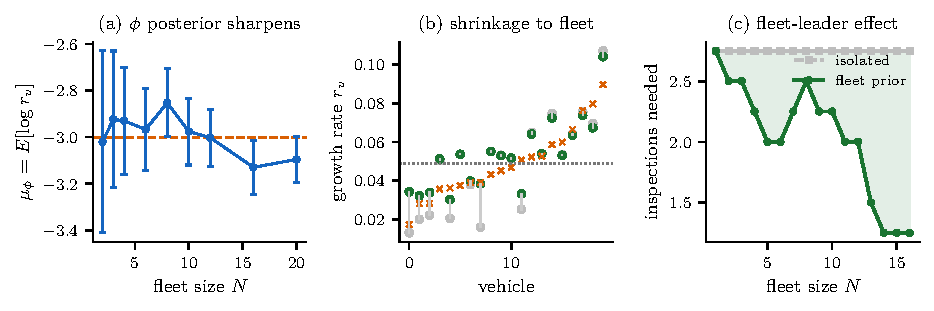
\includegraphics[width=\textwidth]{fleet_learning.pdf}
    \end{column}
    \begin{column}{0.45\textwidth}\footnotesize
      Conjugate-Gibbs partial pooling over a synthetic fleet ($N{=}20$, $F{=}30$):
      \begin{itemize}
        \item recovers $\varphi$: $\mathbb E[\mu]{=}{-}3.10$ (true $-3.0$),
              $\mathbb E[\sigma]{=}0.44$ (true $0.45$)
        \item prior SD sharpens $0.39\!\to\!0.10$
        \item fleet-leader: stable clearance in $\mathbf{1.25}$ vs $\mathbf{2.75}$ inspections
      \end{itemize}
    \end{column}
  \end{columns}
\end{frame}

% --- A13 ---
\begin{frame}{A13 --- Stage-5 multi-objective design (Pareto)}
  \begin{columns}[T]
    \begin{column}{0.55\textwidth}
      \centering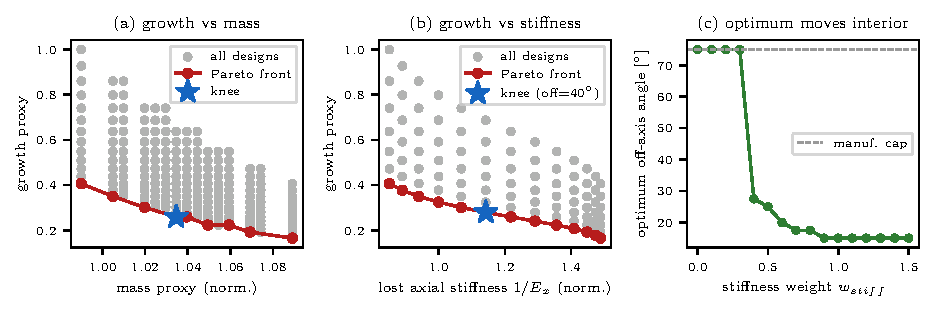
\includegraphics[width=\textwidth]{design_feedback_pareto.pdf}
    \end{column}
    \begin{column}{0.45\textwidth}\footnotesize
      Growth vs.\ mass / axial-stiffness ($A_{11}$) / bending ($D_{11}$):
      \begin{itemize}
        \item single growth objective rails off-axis to the manufacturable cap
        \item competing CLT objectives restore an interior optimum (knee $\sim$$40^\circ$)
        \item optimal angle $75^\circ\!\to\!15^\circ$ as stiffness weight grows
      \end{itemize}
      (sensitivity to uncalibrated constants: main deck.)
    \end{column}
  \end{columns}
\end{frame}

% --- A14 ---
\begin{frame}{A14 --- Differentiable inversion (Keio bridge)}
  \begin{columns}[T]
    \begin{column}{0.5\textwidth}
      \centering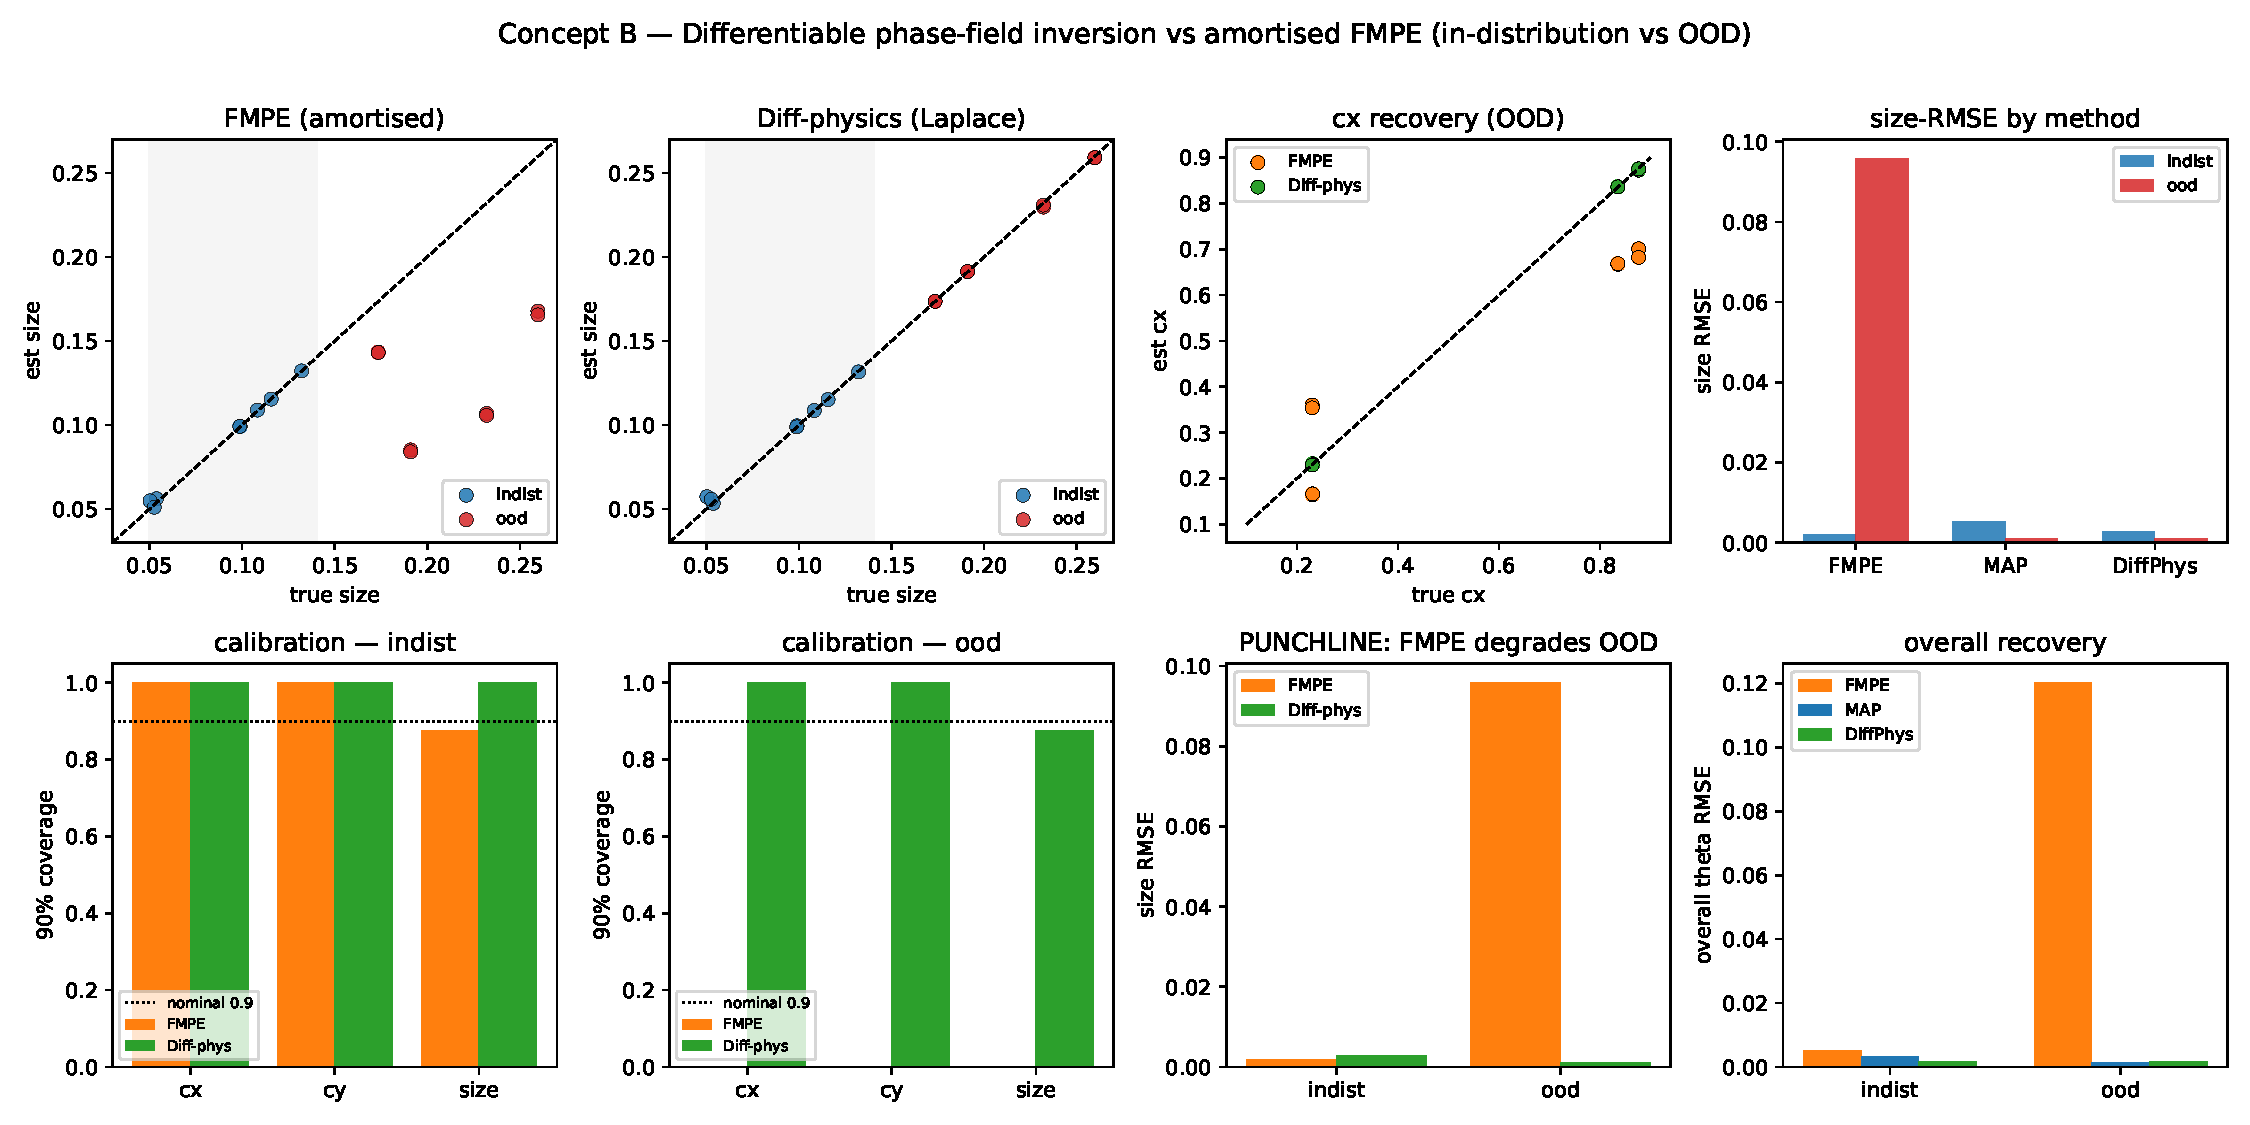
\includegraphics[width=\textwidth]{diff_inversion.pdf}
    \end{column}
    \begin{column}{0.5\textwidth}\footnotesize
      JAX AT2 forward, FD-verified gradient ($3\times10^{-7}$); Laplace posterior
      $\Sigma=\sigma^2(J^\top J+\Lambda)^{-1}$, no labelled pairs.
      \begin{itemize}
        \item amortised collapses OOD ($\sim$25$\times$, $0$ coverage)
        \item differentiable-physics invariant
        \item FNO-as-forward: MAP+Laplace $530\text{s}\!\to\!12\text{s}$ ($43\times$)
      \end{itemize}
      $\Rightarrow$ the cheap forward TMCMC needs (Keio Phase-3).
    \end{column}
  \end{columns}
\end{frame}

% --- A15 ---
\begin{frame}{A15 --- Data provenance and honesty}
  \footnotesize
  \begin{itemize}
    \item \real: interstage TSA full-field (Kojima, CPB 2025 --- \alert{co-author /
          consent gated}); fairing long-term + impact guided waves (OGW);
          SRB-3 AE (4TU CC0); 4TU DCB fatigue.
    \item \synth: phase-field forward (representative $G_c,\ell,\beta$, fatigue);
          synthetic fleet; decision-UQ oracle = exact FD physics.
    \item Reproducibility: $\sim$250 unit tests, one-command end-to-end run,
          MMS / mesh / SNR / economic-sensitivity studies; figures script-generated.
    \item \alert{Open gap:} no real life-test of the prognosis$\to$clearance$\to$fleet chain.
  \end{itemize}
\end{frame}

\end{document}
